\documentclass[border=6pt]{standalone}
\usepackage{tikz}
\usetikzlibrary{arrows.meta,positioning,calc}
\begin{document}
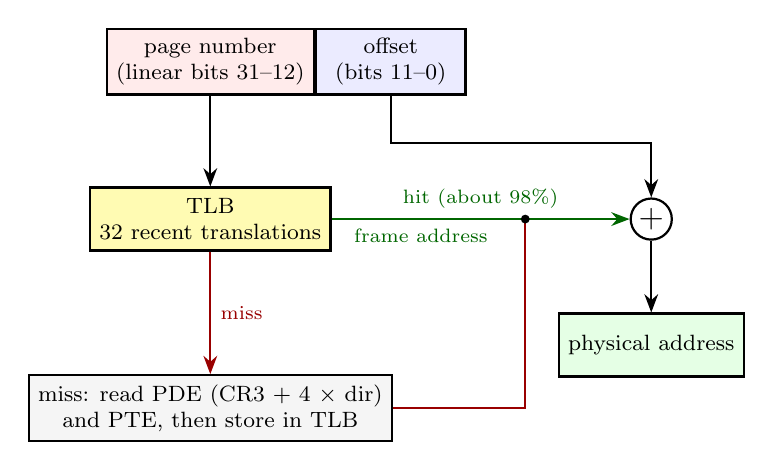
\begin{tikzpicture}[>=Stealth,font=\small,
 b/.style={draw,thick,align=center,font=\footnotesize,minimum height=0.8cm}]
\node[b,fill=red!8,minimum width=2.6cm] (pg) at (0,0) {page number\\(linear bits 31--12)};
\node[b,fill=blue!8,minimum width=1.9cm,right=0pt of pg] (of) {offset\\(bits 11--0)};
\node[b,fill=yellow!30,minimum width=3.0cm] (tlb) at (0,-2.0) {TLB\\32 recent translations};
\draw[->,thick] (pg.south) -- (tlb.north);
\node[circle,draw,thick,inner sep=1pt,font=\large] (add) at (5.6,-2.0) {$+$};
\draw[->,thick,green!40!black] (tlb.east) -- (add.west) node[midway,above,font=\scriptsize]{hit (about 98\%)} node[pos=0.3,below,font=\scriptsize]{frame address};
\draw[->,thick] (of.south) |- ++(0,-0.6) -| (add.north);
\node[b,fill=green!10] (ph) at (5.6,-3.6) {physical address};
\draw[->,thick] (add.south) -- (ph.north);
\node[b,fill=gray!8,minimum width=3.6cm] (walk) at (0,-4.4) {miss: read PDE (CR3 + 4 $\times$ dir)\\and PTE, then store in TLB};
\draw[->,thick,red!60!black] (tlb.south) -- (walk.north) node[midway,right,font=\scriptsize]{miss};
\draw[thick,red!60!black] (walk.east) -| (4.0,-2.0);
\fill (4.0,-2.0) circle (1.6pt);
\end{tikzpicture}
\end{document}
